% Archivo generado automáticamente con los problemas
\section*{Problems}
Sección: 10_Spinors
Páginas: 200-202
Contenido:
10.1 We saw that the Dirac equation predicted that there is interaction between the elec-
tron spin and the magnetic field, ⃗S ⃗B, with strength μB =
ℏc
2me . When the electron
has angular momentum ⃗L, such as in an atomic orbital, there is also a ⃗B⃗L interaction
and a spin-orbit coupling ⃗S⃗L. The Dirac equation (along with symmetry arguments)
predicts the strength of all three interactions, as well as other corrections. To see the
effect of these terms on the hydrogen atom, we have to take the non-relativistic limit.
(a) For the Schr¨odinger equation, we need the Hamiltonian, not the Lagrangian.
Find the Dirac Hamiltonian by writing the Dirac equation as i∂tψ = HDψ.
Write the Hamiltonian in terms of momenta pi rather than derivatives ∂i.
(b) Calculate (HD + eA0)2 in the Weyl representation for ψ = (ψLψR). Leave in
terms of σi, pi and Ai. Put back in the factors of c and ℏ, keeping the charge e
dimensionless.
(c) Now take the square root of this result and expand in 1
c, subtracting off the zero-
point energy mc2, i.e. compute H = HD −mc2 to order c0. Looking at the σi
term, how big are the electron’s electric and magnetic dipole moments?
(d) The size of the terms in this Hamiltonian are only meaningful because the spin
and angular momentum operators have the same normalization. Check the nor-
malization of the angular momentum operators Li = εijkxjpk and the spin
operators Si =
1
2σi
by showing that they both satisfy the rotation algebra:
[Ji, Jj] = iεijkJk.
(e) The gyromagnetic ratio, ge (sometimes called the g-factor), is the relative size
of the ⃗S ⃗B and ⃗L ⃗B interactions. Choose a constant magnetic field in the z direc-
tion, then isolate the BzLz coupling in H. Extract the electron gyromagnetic
ratio ge by writing the entire coupling to the magnetic field in the Hamilto-
nian as μBBz(Lz + geSz) = Bzμz, with ⃗μ ≡μB(⃗L + ge⃗S). How could you
experimentally measure ge (e.g. with spectroscopy of the hydrogen atom)?
(f) In spherical coordinates, the Schr¨odinger equation has a ⃗L2 term. With spin,
you might expect that this becomes ⃗L⃗μ = μB(⃗L2 +ge⃗L⃗S), making the ⃗L⃗S term
proportional to the g-factor. This is wrong. It misses an important relativistic
effect, Thomas precession. It is very hard to calculate directly, but easy to calcu-
late using symmetries. With no magnetic field, the atom, with spin included, is
still rotationally invariant. Which of ⃗J = ⃗L + ⃗S or ⃗μ = ⃗L + ge⃗S is conserved
182
Spinors
(i.e. commutes with ⃗H)? Using this result, how does the spin-orbit coupling
depend on ge?
(g) There are additional relativistic effects coming from the Dirac equation. Expand
the Dirac equation to next order in 1
c2 , producing a term that scales as ⃗p4.
(h) Now let us do some dimensional analysis – there is only one scale me. Show that
the electron’s Compton wavelength, the classical electron radius, re, the Bohr
radius, a0, and the inverse-Rydberg constant, Ry−1, are all me times powers of
αe. Are the splittings due to the p4 term fine structure (ΔE ∼α2
eE), hyperfine
structure (ΔE ∼α4
eE) or something else? [Hint: write out a formula for the
energy shift using time-dependent perturbation theory, then see which of the
above length scales appears.]

10.2 In this problem you will construct the finite-dimensional irreducible representations
of SU(2). By definition, such a representation is a set of three n × n matrices τ1, τ2
and τ3 satisfying the algebra of the Pauli matrices [τi, τj] = iεijkτk. It is also helpful
to define the linear combinations τ ± = τ 1 ± iτ 2.
(a) In any such representation we can diagonalize τ3. Its eigenvectors are n complex
vectors Vj with τ3Vj = λjVj. Show that τ +Vj and τ −Vj either vanish or are
eigenstates of τ3 with eigenvalues λj + 1 and λj −1 respectively.
(b) Prove that exactly one of the eigenstates Vmax of τ3 must satisfy τ +Vmax = 0.
The eigenvalue λmax = j of Vmax is known as the spin. Similarly, there will be
an eigenvector Vmin of τ3 with τ −Vmin = 0.
(c) Since there are a finite number of eigenvectors, Vmin = (τ −)N Vmax for some
integer N. Prove that N = 2J so that n = 2J + 1.
(d) Construct explicitly the five-dimensional representation of SU(2).

10.3 Derive Eqs. (10.141) and (10.142):
(a) gμνσα ˙α
μ σβ ˙β
ν
= 2εαβε ˙α ˙β,
(b) εαβε ˙α ˙βσμβ ˙β = ¯σμ
˙αα.

10.4 Majorana representation.
(a) Write out the form of the Lorentz generators in the Majorana representation.
(b) Compute ⃗J2 in the Majorana representation, the left-handed Weyl representation
and 4-vector representation. How do you interpret the eigenvalues of ⃗J2?
(c) Calculate γ5 = iγ0γ1γ2γ3 in the Majorana representation.

10.5 Supersymmetry.
(a) Show that the Lagrangian
L = ∂μφ⋆∂μφ + χ†i¯σ∂χ + F ⋆F + mφF + i
2mχT σ2χ + h.c.
(10.143)
is invariant under
δφ = −iεT σ2χ,
(10.144)
δχ = ϵF + σμ∂μφσ2ϵ⋆,
(10.145)
δF = −iϵ†¯σμ∂μχ,
(10.146)
where ϵ is an infinitesimal spinor, χ is a spinor, and F and φ are scalars. All
spinors anticommute. σ2 is the second Pauli spin matrix.
Problems
183
(b) The field F is an auxiliary field, since it has no kinetic term. A useful trick for
dealing with auxiliary fields is to solve their equations of motion exactly and
plug the result back into the Lagrangian. This is called integrating out a field.
Integrate out F to show that φ and χ have the same mass.
(c) Auxiliary fields such as F act like Lagrange multipliers. One reason to keep the
auxiliary fields in the Lagrangian is because they make symmetry transforma-
tions exact at the level of the Lagrangian. After the field has been integrated
out, the symmetries are only guaranteed to hold if you use the equations of
motion. Still using δφ = iεT σ2χ, what is the transformation of χ that makes the
Lagrangian in (b) invariant, if you are allowed to use the equations of motion?

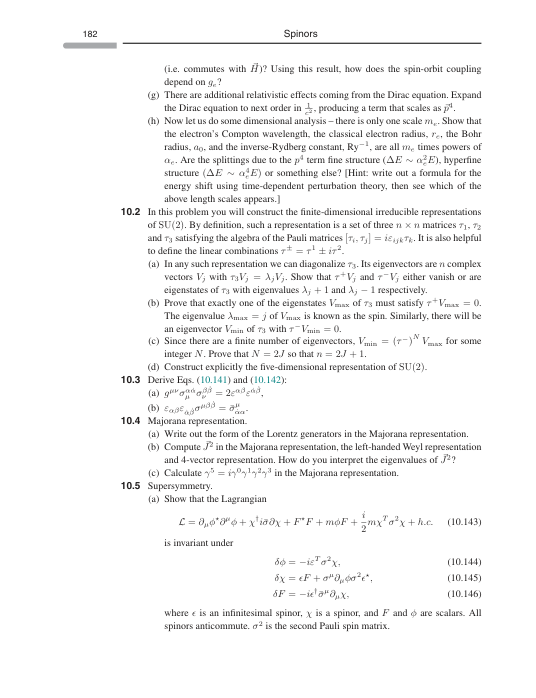
\includegraphics{./figs/10_Spinors_page_202.png}

---

